\chapter{Solution of the equations}\label{CHAP_SOL}

\footnote{This chapter corresponds to section 3 and appendices B and C of~\citep{velasco2019knosos}.}
In this chapter, we provide an overview of how equations~(\ref{EQ_DKEFINAL}) and (\ref{EQ_QNFINAL}) are solved. We first give an explicit expression for equation~(\ref{EQ_DKEFINAL}) in \S\ref{SEC_FINALDKE} and we discuss how to calculate its bounce-averaged coefficients in \S\ref{SEC_COEFFICIENTS}. We then devote \S\ref{SEC_GRID} to build the grid in which we will evaluate the distribution function, and \S\ref{SEC_SOLDKE} to discuss the discretization of the equation. Finally, the solution of quasineutrality, equation  (\ref{EQ_QNFINAL}), is addressed in \S\ref{SEC_SOLQN}.

\section{Final expression of the  drift-kinetic equation}\label{SEC_FINALDKE}

Using the expressions of the pitch-angle scattering collision operator described in equation~(\ref{EQ_COLOP}) and of the magnetic and $E\times B$ drifts in \textit{right handed} Boozer coordinates, equation~(\ref{EQ_DKEFINAL}) can be written in terms of a few bounce integrals:
\begin{eqnarray}
\left(I_{v_{M,\alpha}} (\alpha,\lambda)+\frac{1}{v_{d,b}}I_{v_E,\alpha}(\alpha,\lambda)\right)\partial_\alpha g_b &+& \left( I_{v_{M,\psi}}(\alpha,\lambda)+\frac{1}{v_{d,b}}I_{v_{E,\psi}}(\alpha,\lambda)\right) F_{M,b}\Upsilon_b\nonumber \\
&=& \frac{\nu_{\lambda,b}}{v_{d,b}} \partial_\lambda\left[ I_\nu(\alpha,\lambda) \partial_\lambda g_b\right]\,,
\label{EQ_NDKE}
\end{eqnarray}
with
\begin{eqnarray}
v_{d,b}&\equiv&\frac{m_bv^2}{Z_be}\,,\nonumber\\
I_{v_{E,\alpha}}&=&\Psi_t'\partial_\psi\varphi_0\int_{l_{b_1}}^{l_{b_2}} \frac{\mathrm{d}l}{\sqrt{1-\lambda B}}\,,\nonumber\\
I_{v_{M,\alpha}}&=&\int_{l_{b_1}}^{l_{b_2}}\frac{\mathrm{d}l }{\sqrt{1-\lambda B}}\left(1-\frac{\lambda B}{2}\right)\left[\Psi_t'\frac{\partial_\psi B}{B}+
 \frac{B_\zeta\partial_\theta B - B_\theta\partial_\zeta B}{B|B_\zeta+\iota B_\theta|}\zeta\partial_\psi \iota\right]\,,\nonumber\\
I_{v_{E,\psi}}&=&\int_{l_{b_1}}^{l_{b_2}} \frac{\mathrm{d}l}{\sqrt{1-\lambda B}}\frac{B_\theta\partial_\zeta \varphi_1 - B_\zeta\partial_\theta \varphi_1}{|B_\zeta+\iota B_\theta|}\,,\nonumber\\
I_{v_{M,\psi}}&=&\int_{l_{b_1}}^{l_{b_2}} \frac{\mathrm{d}l }{\sqrt{1-\lambda B}}\left(1-\frac{\lambda B}{2}\right)\frac{B_\theta\partial_\zeta B - B_\zeta\partial_\theta B}{B|B_\zeta+\iota B_\theta|}\,,\nonumber\\
I_\nu&=&\int_{l_{b_1}}^{l_{b_2}} \mathrm{d}l\frac{\lambda\sqrt{1-\lambda B}}{B}\,.
\label{EQ_BINT}
\end{eqnarray}
where $B_\psi$, $B_\theta$ and $B_\zeta$ are the covariant components of $\mathbf{B}$, and $B_\psi=0$ in the low-$\beta$ approximation. We note that only $v_{d,b}$, $\nu_{\lambda,b}$, $F_{M,b}$ and $\Upsilon_b$ depend on the species: the bounce-integrals are only determined by the magnetic configuration and the electrostatic potential. {The magnetic shear appears explicitly  in $I_{v_{M,\alpha}}$.}

Equation~(\ref{EQ_NDKE}) is a differential equation in two variables only, $\alpha$ and $\lambda$, which is the origin of the fast performance of~\KNOSOS~that will be demonstrated in chapter~\ref{CHAP_EX}. The radial coordinate $\psi$ is a parameter, since we are solving radially local equations; $v$ is a parameter as well, since $\varphi_1\ll \varphi_0$; and finally $l$ has disappeared since the coefficients are bounce-averages of certain quantities. The calculation of these coefficients is described in \S\ref{SEC_COEFFICIENTS}.

%%%%%%%%%%%%%%%%%%%%%%%%%%%%%%%%%%%%%%%%%%%%%%%%%%%%%%%%%%%%%%%%%%%%%%%%%%%%%%%%%%%%%%%%%%%%%%%%%%%%%%%%%%%%%%%%%%%

\section{Calculation of the coefficients of the drift-kinetic equation}\label{SEC_COEFFICIENTS}

%%%%%%%%%%%%%%%%%%%%%%%%%%%%%%%%%%%%%%%%%%%%%%%%%%%%%%%%%%%%%%%%%%%%%%%%%%%%%%%%%%%%%%%%%%%%%%%%%%%%%%%%%%%%%%%%%%%

The integrals in $l$ are done using an extended midpoint rule \citep[see e.g.][subroutine {\ttfamily midpnt}]{numericalrecipes}. This open formula is appropriate for integrals that are improper in the sense that they have an integrable singularity at the integration limits. This is our case, since by definition $\lambda B(l_{b_1}) = \lambda B(l_{b_2}) =1$. The number of points that we use is not pre-defined: starting from being one, it is tripled until the integral converges. %Specifically, until the relative variation of the numerical integral is smaller than \vlink{PREC\_BINT}.

Let us now note that integrals such as those of equations~(\ref{EQ_BINT}) may be difficult to converge if the numerator does not go to zero in the integration limits, or it does, but slower than the denominator. This may happen, first, if $\lambda$ is such that $l_{b_1}$ or $l_{b_2}$ are close to a point $l_T$ where $B(l)$ has a local maximum $B(l_T)$ for fixed $\alpha$; second, if the interval ($l_{b_1},l_{b_2}$) contains a point $l_B$ where $B(l)$ has a local maximum and $\lambda$ is close to $\lambda_B\equiv 1/B(l_B)$. In such cases, $I(\lambda)$ may become very large; if the inverse of $\lambda$  is equal to the corresponding maximum of $B$, the integral diverges logarithmically.  We can physically identify these situations in the example of figure~\ref{FIG_ORBIT}: divergences happen at \textit{bifurcations}, where orbits go from being trapped in a particular  region in $l$ to be trapped, for smaller $\lambda$, in a wider region (the boundary between passing and trapped particles is a particular case of this).  

One can ease the convergence, and thus make the calculation faster, by removing the divergence and solving it analytically as explained in Appendix C of~\citep{calvo2017sqrtnu}. This is described more in detail in the next subsection. Another subsection discusses how the fact that field lines are straight in magnetic coordinates is used to accelerate the evaluation of the magnetic field strength at each point ($\alpha, l$) without loss of accuracy.

%%%%%%%%%%%%%%%%%%%%%%%%%%%%%%%%%%%%%%%%%%%%%%%%%%%%%%%%%%%%%%%%%%%%%%%%%%%%%%%%%%%%%%%%%%%%%%%%%%%%%%%%%%%%%%%%%%%

\subsection{Analytical calculation of the divergences of some bounce-integrals}\label{SEC_DIV}

%%%%%%%%%%%%%%%%%%%%%%%%%%%%%%%%%%%%%%%%%%%%%%%%%%%%%%%%%%%%%%%%%%%%%%%%%%%%%%%%%%%%%%%%%%%%%%%%%%%%%%%%%%%%%%%%%%%

In this subsection, we discuss how integrals such as those in equations~(\ref{EQ_BINT}),
\begin{equation} 
I(\lambda)=\int_{l_{b_1}}^{l_{b_2}}\mathrm{d}l\,\frac{f(\lambda,l)}{\sqrt{1-\lambda B(l)}}\,,
\end{equation}
can be computed efficiently by removing the component that diverges close to bifurcations and solving it analytically. Since integration is done at fixed $\alpha$, we ease the notation by not making it explicit that $B$, $f$, and $I$ generally depend on the angular coordinate.
%can be computed efficiently by removing the component that diverges close to bifurcations and solving it analytically if \vlink{REMOVE\_DIV} is set to \true. Since integration is done at fixed $\alpha$, we ease the notation by not making it explicit that $B$, $f$, and $I$ generally depend on the angular coordinate.

We first expand the magnetic field around the bounce point:
\begin{equation} 
B(l)=B(l_{b_1})+\partial_l B|_{l_{b_1}}(l-l_{b_1})+\frac{1}{2}\partial^2_l B|_{l_{b_1}}(l-l_{b_1})^2\,.
\end{equation}
Close to the bounce point, we have
\begin{eqnarray}
\frac{f(l)}{\sqrt{1-\lambda B(l)}} \approx \frac{f(l_{b_1})}{\sqrt{-\lambda (l-l_{b_1}) [\partial_l B|_{l_{b_1}}+\frac{1}{2}\partial^2_l B|_{l_{b_1}}(l-l_{b_1})]}}\,
\end{eqnarray}
since $\lambda B(l_{b_1})=1$. We can proceed exactly in the same way close to $l_{b_2}$, and similarly close to $\lambda_B$: there, $\lambda B(l_B)<1$ and the first derivative $\partial_l B|_{l_B}$ is zero, and we have
\begin{eqnarray}
\frac{f(l)}{\sqrt{1-\lambda B(l)}} \approx \frac{f(l_B)}{\sqrt{-(\lambda-\lambda_B) B(l_B)-\lambda_B\frac{1}{2}\partial^2_l B|_{l_B}(l-l_B)^2}}\,.
\end{eqnarray}
We can then split the integral in three contributions:
\begin{equation} 
I= I_0+I_1+I_2+I_B\,,
\end{equation}
with
\begin{eqnarray}
I_0 &=&  \int_{l_{b_1}}^{l_{b_2}}\mathrm{d}l\,\left(\frac{f(l)}{\sqrt{1-\lambda B(l)}}\right.\nonumber\\
 &-&\frac{f(l_{b_1})}{\sqrt{-\lambda (l-l_{b_1}) [\partial_l B|_{l_{b_1}}+\frac{1}{2}\partial^2_l B|_{l_{b_1}}(l-l_{b_1})]}}\nonumber\\
 &-&\frac{f(l_{b_2})}{\sqrt{-\lambda (l-l_{b_2}) [\partial_l B|_{l_{b_2}}+\frac{1}{2}\partial^2_l B|_{l_{b_2}}(l-l_{b_2})]}}\nonumber\\
 &-&\left.\frac{f(l_B)}{\sqrt{-(\lambda-\lambda_B) B(l_B)-\lambda_B\frac{1}{2}\partial^2_l B|_{l_B}(l-l_B)^2}}\right)\,,
\end{eqnarray}
whose integrand does not diverge anywhere and
\begin{eqnarray} 
I_1 &=&  \int_{l_{b_1}}^{l_{b_2}}\mathrm{d}l\,\frac{f(l)}{\sqrt{-\lambda (l-l_{b_1}) [\partial_l B|_{l_{b_1}}+\frac{1}{2}\partial^2_l B|_{l_{b_1}}(l-l_{b_1})]}}\,,\nonumber\\
I_2 &=&  \int_{l_{b_1}}^{l_{b_2}}\mathrm{d}l\,\frac{f(l)}{\sqrt{-\lambda (l-l_{b_2}) [\partial_l B|_{l_{b_2}}+\frac{1}{2}\partial^2_l B|_{l_{b_2}}(l-l_{b_2})]}}\,,\nonumber\\
I_B &=&  \int_{l_{b_1}}^{l_{b_2}}\mathrm{d}l\,\frac{f(l_B)}{\sqrt{-(\lambda-\lambda_B) B(l_B)-\lambda_B\frac{1}{2}\partial^2_l B|_{l_B}(l-l_B)^2}}\,,
\end{eqnarray}
which can be solved analytically. The integral close to the bottom is
\begin{eqnarray} 
I_B &=&  \sqrt{\frac{-2}{\lambda_B\partial^2_l B|_{l_B}}} \left[\mathrm{ln}\left(x+\sqrt{x^2+\frac{2(\lambda-\lambda_B) B(l_B)}{\lambda_B\partial^2_l B|_{l_B}}}\right)\right]^{l_B-l_{b_1}}_0\nonumber\\
&+&  \sqrt{\frac{-2}{\lambda_B\partial^2_l B|_{l_B}}} \left[\mathrm{ln}\left(x+\sqrt{x^2+\frac{2(\lambda-\lambda_B) B(l_B)}{\lambda_B\partial^2_l B|_{l_B}}}\right)\right]_0^{l_{b_2}-l_B}\,.
\end{eqnarray}

For the other two integrals, if $\partial^2_l B|_{l_{b_1}}<0$ and $\partial^2_l B|_{l_{b_2}}<0$, the solution is
\begin{eqnarray} 
I_1 &=&  \sqrt{\frac{-2}{\lambda\partial^2_l B|_{l_{b_1}}}}  \times\nonumber\\
& &\hskip-0.5cm \left[\mathrm{ln}\left(2\lambda\sqrt{\frac{\partial^2_l B|_{l_{b_1}}}{-2}}\sqrt{ -\partial_l B|_{l_{b_1}}x -\frac{1}{2}\partial^2_l B|_{l_{b_1}}x^2} -\lambda \partial^2_l B|_{l_{b_1}} x -\lambda\partial_l B|_{l_{b_1}}\right)\right]_0^{l_{b_2}-l_{b_1}}\,,\nonumber\\
I_2 &=&  \sqrt{\frac{-2}{\lambda\partial^2_l B|_{l_{b_2}}}}  \times\nonumber\\
& &\hskip-0.5cm\left[\mathrm{ln}\left(2\lambda\sqrt{\frac{\partial^2_l B|_{l_{b_2}}}{-2}}\sqrt{ -\partial_l B|_{l_{b_2}}x -\frac{1}{2}\partial^2_l B|_{l_{b_2}}x^2} -\lambda \partial^2_l B|_{l_{b_2}} x -\lambda\partial_l B|_{l_{b_2}}\right)\right]_{l_{b_1}-l_{b_2}}^0\hskip-0.5cm.
\end{eqnarray} 
These expressions are useful (in the sense of removing large analytical contributions to $I$) close enough to a bifurcation, where they can significantly accelerate the convergence of equations~(\ref{EQ_BINT}), but they are in principle valid for any $\lambda$ (far from bifurcations,  when $\partial^2_l B|_{l_{b_1}}$ is positive, the expression within the square-root may become negative and cannot be used).

%Figure~\ref{FIG_INT} shows the integrands of $I$, $I_1$, $I_2$ and $I_B$ for one particular case of the calculation of the bounce-averaged coefficients of equation~(\ref{EQ_BINT}). It is shown that, by calculating anallitically $I_1$, $I_2$ and $I_B$. For values of $1/\lambda$ close enough to the corresponding maximum of $B$, the , the calculation of 
%It works better the more optimized the stellarator, as we learn from the figure: this particular orbit passes close not only to the relative maxima of $B$ corresponding to $\lambda_B$ but also close to other relative maxima that we ignore. In some cases, resolving numerically the large contribution of these maxima to the integral may get as computationally hard as the contributions that we have removed. These situations will be more frequent in the $\sqrt{\nu}$ regime (where the boundary layer between trapped and passing particles need to be well described~\citep{calvo2017sqrtnu}) than in the 1/$\nu$ or superbanana-plateau regimes.

%%%%%%%%%%%%%%%%%%%%%%%%%%%%%%%%%%%%%%%%%%%%%%%%%%%%%%%%%%%%%%%%%%%%%%%%%%%%%%%%%%%%%%%%%%%%%%%%%%%%%%%%%%%%%%%%%%%

\subsection{Evaluation of the magnetic field strength along a field line}\label{SEC_DELTA}

%%%%%%%%%%%%%%%%%%%%%%%%%%%%%%%%%%%%%%%%%%%%%%%%%%%%%%%%%%%%%%%%%%%%%%%%%%%%%%%%%%%%%%%%%%%%%%%%%%%%%%%%%%%%%%%%%%%

The fact that field lines are straight in magnetic coordinates can also be used to speed up the calculation of the coefficients of the drift-kinetic equation. We describe how in this subsection. 
%The fact that field lines are straight in magnetic coordinates can also be used to speed up the calculation of the coefficients of the drift-kinetic equation if \vlink{DELTA}  is set to \true. We describe how in this subsection. 

The bounce-integrals are done, using the algorithm mentioned in \S\ref{SEC_COEFFICIENTS}, by following field lines using a fixed step in the Boozer angles given by $\Delta\zeta$ and $\Delta\theta=\iota\Delta\zeta$. After each step, the magnetic field can be calculated without loss of accuracy from its Fourier components
\begin{eqnarray}
B(\theta,\zeta)&=&\sum_{m,n}  B_{m,n}^{(c)}(\cos[m\theta+nN\zeta]\nonumber\\
  &+&\sum_{m,n}  B_{m,n}^{(s)}(\cos[m\theta+nN\zeta]\,,\nonumber\\
B(\theta+\Delta\theta,\zeta+\Delta\zeta)&=&\sum_{m,n} B_{m,n}^{(c)}\cos[m(\theta+\Delta\theta)+nN(\zeta+\Delta\zeta)]\nonumber\\
&+&\sum_{m,n} B_{m,n}^{(s)}\sin[m(\theta+\Delta\theta)+nN(\zeta+\Delta\zeta)]\,,\nonumber\\
B(\theta+2\Delta\theta,\zeta+2\Delta\zeta)&=&\sum_{m,n} B_{m,n}^{(c)}\cos[m(\theta+2\Delta\theta)+nN(\zeta+2\Delta\zeta)]\nonumber\\
&+&\sum_{m,n} B_{m,n}^{(s)}\sin[m(\theta+2\Delta\theta)+nN(\zeta+2\Delta\zeta)]\,,\nonumber\\
...
\end{eqnarray}
Instead of calculating the cosines at every angular position, we can precalculate a few sines and cosines, $\cos(m\theta+nN\zeta)$, $\sin(m\theta+nN\zeta)$, $\cos(m\Delta\theta+nN\Delta\zeta)$ and $\sin(m\Delta\theta+nN\Delta\zeta)$, and use well-known trigonometric identities to iterate:
 \begin{eqnarray}
\cos[m(\theta+\Delta\theta)+nN(\zeta+\Delta\zeta)] & = &\cos(m\theta+nN\zeta)\cos(m\Delta\theta+nN\Delta\zeta)\nonumber\\
&-& sin(m\theta+nN\zeta)\sin(m\Delta\theta+nN\Delta\zeta)\,,\nonumber\\
\sin[m(\theta+\Delta\theta)+nN(\zeta+\Delta\zeta)] & =& \cos(m\theta+nN\zeta)\sin(m\Delta\theta+nN\Delta\zeta)\nonumber\\
&+& \sin(m\theta+nN\zeta)\cos(m\Delta\theta+nN\Delta\zeta)\,,
\end{eqnarray}
and
 \begin{eqnarray}
\cos[m(\theta+2\Delta\theta)+nN(\zeta+2\Delta\zeta)] & =& \cos[m(\theta+\Delta\theta)+nN(\zeta+\Delta\zeta)]\cos(m\Delta\theta+nN\Delta\zeta)\nonumber\\
&-& sin[m(\theta+\Delta\theta)+nN(\zeta+\Delta\zeta)]\sin(m\Delta\theta+nN\Delta\zeta)\,,\nonumber\\
\sin[m(\theta+2\Delta\theta)+nN(\zeta+2\Delta\zeta)] & = &\cos[m(\theta+\Delta\theta)+nN(\zeta+\Delta\zeta)]\sin(m\Delta\theta+nN\Delta\zeta)\nonumber\\
&+& \sin[m(\theta+\Delta\theta)+nN(\zeta+\Delta\zeta)]\cos(m\Delta\theta+nN\Delta\zeta)\,\nonumber\\
\end{eqnarray}
and so on.



%%%%%%%%%%%%%%%%%%%%%%%%%%%%%%%%%%%%%%%%%%%%%%%%%%%%%%%%%%%%%%%%%%%%%%%%%%%%%%%%%%%%%%%%%%%%%%%%%%%%%%%%%%%%%%%%%%%

\section{Spatial and velocity grid}\label{SEC_GRID}

%%%%%%%%%%%%%%%%%%%%%%%%%%%%%%%%%%%%%%%%%%%%%%%%%%%%%%%%%%%%%%%%%%%%%%%%%%%%%%%%%%%%%%%%%%%%%%%%%%%%%%%%%%%%%%%%%%%

In \S\ref{SEC_COEFFICIENTS} we have seen how the integrals of equations~(\ref{EQ_BINT}) are calculated. These integrals will be evaluated at the points ($\alpha,\lambda$) in which we want to determine the distribution function $g_b$. The selection of these points constitute the subject of this section.

Let us start with the spatial grid. We have seen that $\psi$ is a parameter, and $l$ does not appear in the bounce-averaged drift-kinetic equation, which leaves us with the field line label $\alpha$. There are, however, two complications: first, at a given $\alpha$ and $\lambda$, several wells may exist (in other words, several pairs of $l_{b_1}$ and $l_{b_2}$), which means that we need to use an integer label $w$ for them (as we will discuss more in detail in the following section). Second, even if $g_b$ does not depend on $l$, its integrals over velocities (needed e.g. to compute $\varphi_1$, see equation~(\ref{EQ_QNFINAL})) do, so we must define a two-dimensional angular grid. As a general rule, when doing so, we try to minimize the number of points at which $g_b$ needs to be solved, in order to save computing resources. With this in mind, we make use of periodicity and align the grid points with the field lines. The grid points are also aligned with $\zeta=0$.

\begin{figure}\vskip-1.5cm
\centerline{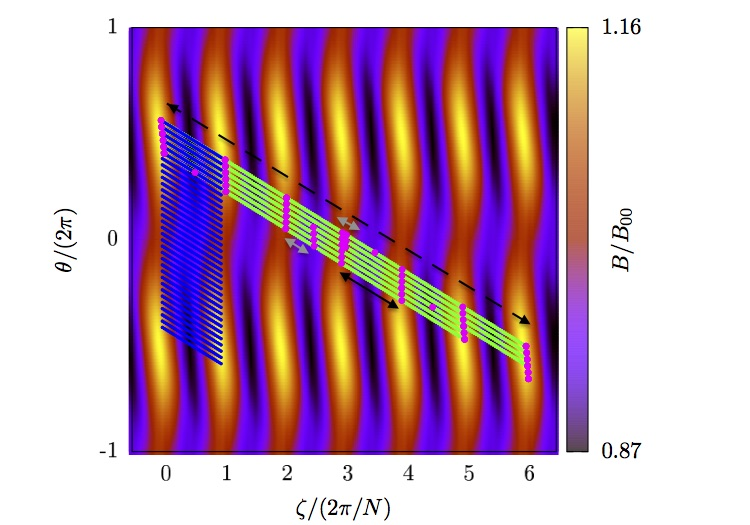
\includegraphics[angle=0,width=\columnwidth]{figures/ang_grid.jpg}}
\centerline{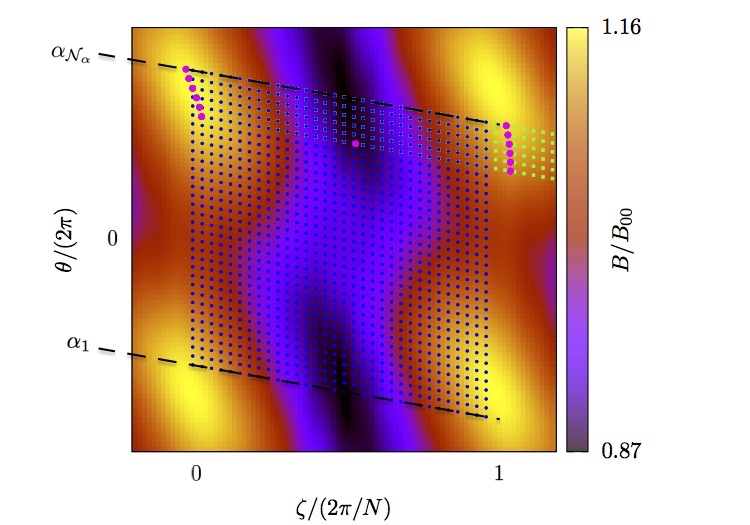
\includegraphics[angle=0,width=\columnwidth]{figures/ang_grid_zoom.jpg}}
\caption{Construction of the angular grid (see text) for a flux-surface of W7-X (top); zoom (bottom).}
\label{FIG_GRID}
\end{figure}

We use figure~\ref{FIG_GRID} (top), which shows one example of stellarator flux surface (the W7-X case discussed in \S\ref{SEC_DKES}) to describe how the angular grid is built. We follow several field lines until they have completed a full poloidal turn. The distance between two consecutive field lines $\Delta\alpha$ is taken to be an integer fraction (one sixth, in the plot) of $2\pi\iota/N$, where $N$ is the number of toroidal periods. This is how the green points are located, with uniform spacing in the toroidal angle. Along the field lines, several maxima of the magnetic field are found, plotted with magenta circles. It is observed that we are dealing with a relatively optimized configuration, in the sense that most trapped particles are so in a major well that coincides with one field period (black continuous arrow). In other words, their bounce points $l_{b_1}$ and $l_{b_2}$ are two consecutive magenta points, separated toroidally by a characteristic angular distance $\sim 2\pi/N$ (smaller for large values of $\lambda$, close to the bottom of the magnetic well). In the example, several ripple wells are found (grey arrows). For small enough values of $\lambda$, trajectories trapped in more than one field-period exist: in this example, particles may move between $\zeta=0$ and $\zeta=6\frac{2\pi}{N}$ (black dashed arrow); trajectories with smaller $\lambda$ (that is, trapped in more than 6 toroidal periods) are ignored in this case; this procedure effectively sets the boundary between passing and trapped particles (following field lines until they have completed more than one poloidal turn would allow us to describe trajectories with smaller $\lambda$,  but this is not necessary in the light of the results of chapter~\ref{CHAP_EX}).

Periodicity allows us to project all these grid points onto the first period. The result is a bidimensional grid in $\alpha$ and $l$, with ${\cal{N}}_\alpha$ and ${\cal{N}}_l$ points in each direction. ${\cal{N}}_\alpha$ is the integer quantity such that ${\cal{N}}_\alpha<\frac{2\pi}{\Delta\alpha}\le{\cal{N}}_\alpha+1$. The ${\cal{N}}_l$ points along the field line are distributed uniformly in the toroidal angle along a toroidal period, and ${\cal{N}}_l$ is the largest power of 2 that is smaller than or equal to ${\cal{N}}_\alpha$. This will be useful for a fast computation of the Fourier transform, needed when solving quasineutrality. Toroidal periodicity is also enforced at the corners of the grid: for instance, in figure~\ref{FIG_GRID} bottom, point $\alpha=\alpha_{{\cal{N}}_\alpha-4}$, $\zeta=0$, is not contained in the wells marked in magenta. Using periodicity, the value of the distribution function at  this point will be taken to be equal to the value at $\alpha=\alpha_1$ and $\zeta=2\pi/N$. The number of points where this has to be done can be minimized by putting one of the corners of the grid close to the global maximum of $B$ on the flux-surface. For each of the nodes of this grid (and for each of the possible values of $\lambda$) the points along the trajectory and the bounce points of particles trapped in one or several field-periods are now clearly identified, and the integrals of equation~(\ref{EQ_BINT}) can be evaluated. 

Let us turn our attention to the velocity grid, where we are using $\lambda$ and $v$ as coordinates. Since we have seen in chapter \ref{CHAP_EQ} that only trapped particles need to be calculated, an obvious choice for the former is a uniform grid\footnote{When the particles are in the $1/\nu$ regime, special attention should be paid to bifurcations, where $g_b$ has discontinuous first $\lambda$-derivatives~\citep{nemov1999neo,calvo2014er}, and a non-uniform grid, adapted to the structure of maxima and minima at fixed $\alpha$, is a more efficient choice~\citep{kernbichler2016neo2}. The same applies to very low collisionalities, when the contribution to the flux is concentrated on very thin $\lambda$ layers. For the wide parameter range that will be studied with~\KNOSOS, the uniform grid is considered appropriate.}, with ${\cal{N}}_\lambda+1$ values between $\lambda_1\equiv 1/B_{max}$ and $\lambda_{{\cal{N}}_\lambda+1}\equiv 1/B_{min}$. The distribution function will not be evaluated at $\lambda_{{\cal{N}}_\lambda+1}$, which will be \textit{ghost} points employed for imposing the boundary conditions at the bottom of the well. When integrating in $\lambda$, we will use the extended trapezoidal rule~\citep[][]{numericalrecipes}.

Finally, $v$ is a parameter in our calculations: equation~(\ref{EQ_NDKE}) will be solved for several values $v_i$ of the velocity and the solution will be numerically integrated in $v$. Since the integrand of equations~(\ref{EQ_VELINT}) contains an exponential coming from the Maxwellian distribution, we will use Gauss-Laguerre of order 64~\citep[][]{numericalrecipes}:
\begin{equation}
\int_0^\infty\,\mathrm{d}(v^2/v_{th,b}^2) f(v^2/v_{th,b}^2) \exp{(-v^2/v^2_{th,b})} \approx \sum_{i=1}^{n} \omega_i f(v_i^2/v_{th,b}^2)\,,
\label{EQ_CONV}
\end{equation}
being $v_{th,b}$ the thermal velocity of species $b$, and $\omega_i$ a set of tabulated real numbers. This procedure requires solving the monoenergetic drift-kinetic equation for $n=64$ values of $v/v_{th,b}$, typically from $\sim 10^{-2}$ to $\sim 10^2$. However, the contribution of the largest $v_i$ to the integral can be usually neglected, and this allows for an important reduction of computing time. Let us finally note that this is a standard and well-tested choice in neoclassics and gyrokinetics~\citep[e.g.][]{velasco2011bootstrap,barnes2019stella}, although other velocity-space discretization methods have been proposed in recent years~\citep{landreman2013intv} that could be easily implemented in~\KNOSOS.

%%%%%%%%%%%%%%%%%%%%%%%%%%%%%%%%%%%%%%%%%%%%%%%%%%%%%%%%%%%%%%%%%%%%%%%%%%%%%%%%%%%%%%%%%%%%%%%%%%%%%%%%%%%%%%%%%%%

\section{Discretization of the drift-kinetic equation}\label{SEC_SOLDKE}

%%%%%%%%%%%%%%%%%%%%%%%%%%%%%%%%%%%%%%%%%%%%%%%%%%%%%%%%%%%%%%%%%%%%%%%%%%%%%%%%%%%%%%%%%%%%%%%%%%%%%%%%%%%%%%%%%%%

In \S\ref{SEC_GRID} we have built a grid in variables $\alpha$ and $\lambda$. Three integers can be used to label any point $(\alpha_i,\lambda_j,w)$ of this grid: $i$ runs from 1 to  ${\cal{N}}_\alpha$,  $j$ from 1 to ${\cal{N}}_\lambda$ and $w=I,II...$ is an integer that labels wells for a given $\alpha$ and $\lambda$. At a given point, we define $g_{i,j,w}\equiv g_b(\alpha_i,\lambda_j,w)$,  $I_{\nu,i,j,w}\equiv I_\nu(\alpha_i,\lambda_j,w)$ and so on (in order to ease the notation, $g_{i,j,w}$ does not contain a species index). The final step in the discretization of the drift-kinetic equation is how we approximate the derivatives of $g_b$ of equation~(\ref{EQ_NDKE}) at each point of this grid.


Let us start with the collision operator, which divided by $ \frac{\nu_{\lambda},b}{v_{d,b}}$ reads
\begin{equation}
\partial_\lambda\left[ I_\nu \partial_\lambda g_b\right]\,,
\label{EQ_COL}
\end{equation}
and can be expanded into two terms
\begin{equation}
\left[ I_\nu \partial^2_\lambda  + (\partial_\lambda I_\nu) \partial_\lambda \right] g_b\,. 
\label{EQ_CO_EXP}
\end{equation}
We represent the $\lambda$ grid at fixed $\alpha$ in figure~\ref{FIG_LAMBDA}. Here, $\lambda_1$ is the boundary between passing and trapped particles. In this example, only one complete well is plotted at $\lambda_2$, labelled $I$. If one moves to larger $\lambda$, a bifurcation appears in the vicinity of $\lambda_{j_0}$, with two wells labelled $I$ and $II$. At a larger value of $\lambda$, there are the bottoms of the wells, where the wells have their minimum magnetic field (different in $I$ than in $II$) and beyond which no orbits are allowed.

 At a generic point, we make use of equation~(\ref{EQ_CO_EXP}) and then employ central finite differences with second-order accuracy
\begin{eqnarray}
\left[ I_\nu \partial^2_\lambda  + (\partial_\lambda I_\nu) \partial_\lambda \right] g_b|_{i,j,w}&=& I_\nu,_{i,j,w} \frac{g_{i,j+1,w}+g_{i,j-1,w}-2g_{i,j,w}}{(\Delta\lambda)^2}\nonumber\\&+&\partial_\lambda I_\nu |_{i,j,w} \frac{g_{i,j+1,w}-g_{i,j-1,w}}{2\Delta\lambda}\,,
\label{EQ_D2LAMBDA}
\end{eqnarray}
with $\Delta\lambda=\lambda_{j+1}-\lambda_j$. Differentiation is done at fixed $\alpha$ and well-label $w$. At a bifurcation, such as the one near $\lambda_{j_0}$ in figure~\ref{FIG_LAMBDA}, we use finite differences with second-order accuracy directly over equation~(\ref{EQ_COL}) and summing over wells,
%with $\Delta\lambda=\lambda_{j+1}-\lambda_j$. Differentiation is done at fixed $\alpha$ and well-label $w$. Nevertheless, equation~(\ref{EQ_D2LAMBDA}) relies on $\partial_\lambda g$ being continuous, which is not fulfilled at bifurcations if the effect of the tangential drift is small. At a bifurcation, such as the one near $\lambda_{j_0}$ in figure~\ref{FIG_LAMBDA}, we use finite differences with second-order accuracy directly over equation~(\ref{EQ_COL}) and summing over wells, 
\begin{eqnarray}
\partial_\lambda\left[ I_\nu \partial_\lambda g_b\right]|_{i,j_0,I}&=& \frac{[I_\nu \partial_\lambda g_b]|_{i,j_0+1,I} +  [I_\nu \partial_\lambda g_b]|_{i,j_0+1,II} -   [I_\nu \partial_\lambda g_b]|_{i,j_0-1,I}}{2\Delta\lambda}\,\nonumber\\
&=& I_\nu,_{i,j_0+1,I}\frac{g_{i,j_0+2,I}-g_{i,j_0,I}}{4(\Delta\lambda)^2}\nonumber\\
&+& I_\nu,_{i,j_0+1,II}\frac{g_{i,j_0+2,II}-g_{i,j_0,I}}{4(\Delta\lambda)^2}\nonumber\\
&-&I_\nu,_{i,j_0-1,I}\frac{g_{i,j_0,I}-g_{i,j_0-2,I}}{4(\Delta\lambda)^2}\,.\label{EQ_DLAMBDABIF}
\end{eqnarray}
This discretization is designed to obtain the expected relation between different values of $\partial_\lambda g$ at the bifurcation for the $1/\nu$ regime~\citep{nemov1999neo,calvo2014er}. Finally, we have two kinds of boundary conditions: one at the boundary between passing and trapped particles, corresponding to equation~(\ref{EQ_CONT2}),
\begin{equation}
g_{i,1,w}=0\,,
\label{EQ_TOP}
\end{equation}
and one at the bottom, corresponding to regularity~\citep{calvo2013er},
\begin{equation}
\partial_\lambda\left[ I_\nu \partial_\lambda g_b\right]|_{i,{\cal{N}}_\lambda,w} = -I_\nu,_{i,{\cal{N}_\lambda}-1,w}\frac{g_{i,{\cal{N}}_\lambda,w}-g_{i,{\cal{N}}_\lambda-2,w}}{4(\Delta\lambda)^2}\,.
\label{EQ_BOTTOM}
\end{equation}
Here we have employed a ghost point $\lambda_{{\cal{N}}_\lambda+1}$ at exactly the bottom of the well, where $I_{\nu,i,{\cal{N}}_\lambda+1,w}=0$. One precision must be made: while in omnigenous magnetic fields the values of the maxima and minima of $B$ are the same when moving in $\alpha$, and equation~(\ref{EQ_BOTTOM}) can be used as such for all $\alpha$, this ceases to be true in a generic stellarator. For instance, the distance from $\lambda_{{\cal{N}_\lambda}}$ to the local bottom will be exactly $\Delta\lambda$ for one field line and smaller elsewhere (it may even happen that the contour condition must not be applied to $\partial_\lambda\left[ I_\nu \partial_\lambda g_b\right]|_{i,{\cal{N}}_\lambda,w}$, but to $\partial_\lambda\left[ I_\nu \partial_\lambda g_b\right]|_{i,j,w}$ with a smaller $j$). This requires introducing straightforward corrections to equations~(\ref{EQ_D2LAMBDA}), (\ref{EQ_DLAMBDABIF}), (\ref{EQ_TOP}) and (\ref{EQ_BOTTOM}).

\begin{figure}
\centering
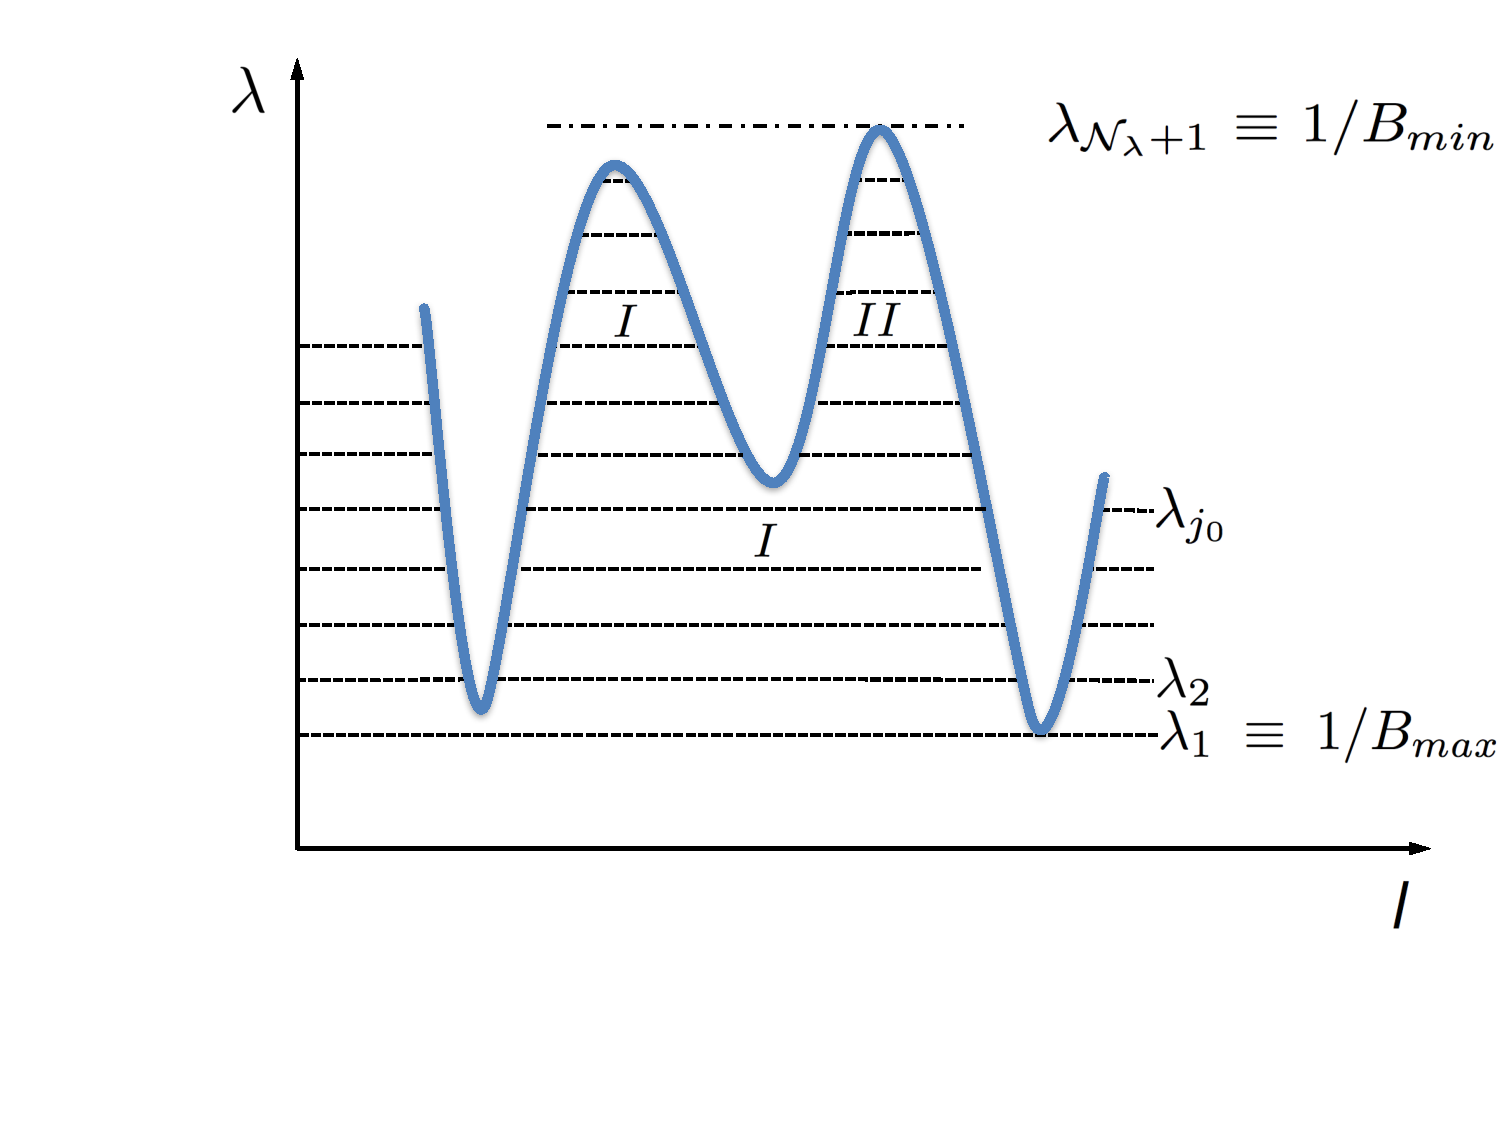
\includegraphics[angle=0,width=0.8\columnwidth]{figures/lambda_l}\
\caption{Sketch of grid in $\lambda$ space at fixed $\alpha$. The collision operator is discretized as in equation~(\ref{EQ_D2LAMBDA}) except at the top ($\lambda_1$) or bottom ($\lambda_{{\cal{N}}_\lambda}$) of the well and at bifurcations (e.g. $\lambda_{j_0}$); there, equations~(\ref{EQ_BOTTOM}),~(\ref{EQ_TOP})  and~(\ref{EQ_DLAMBDABIF}), respectively are used instead.}
\label{FIG_LAMBDA}
\end{figure}

\begin{figure}
\centering
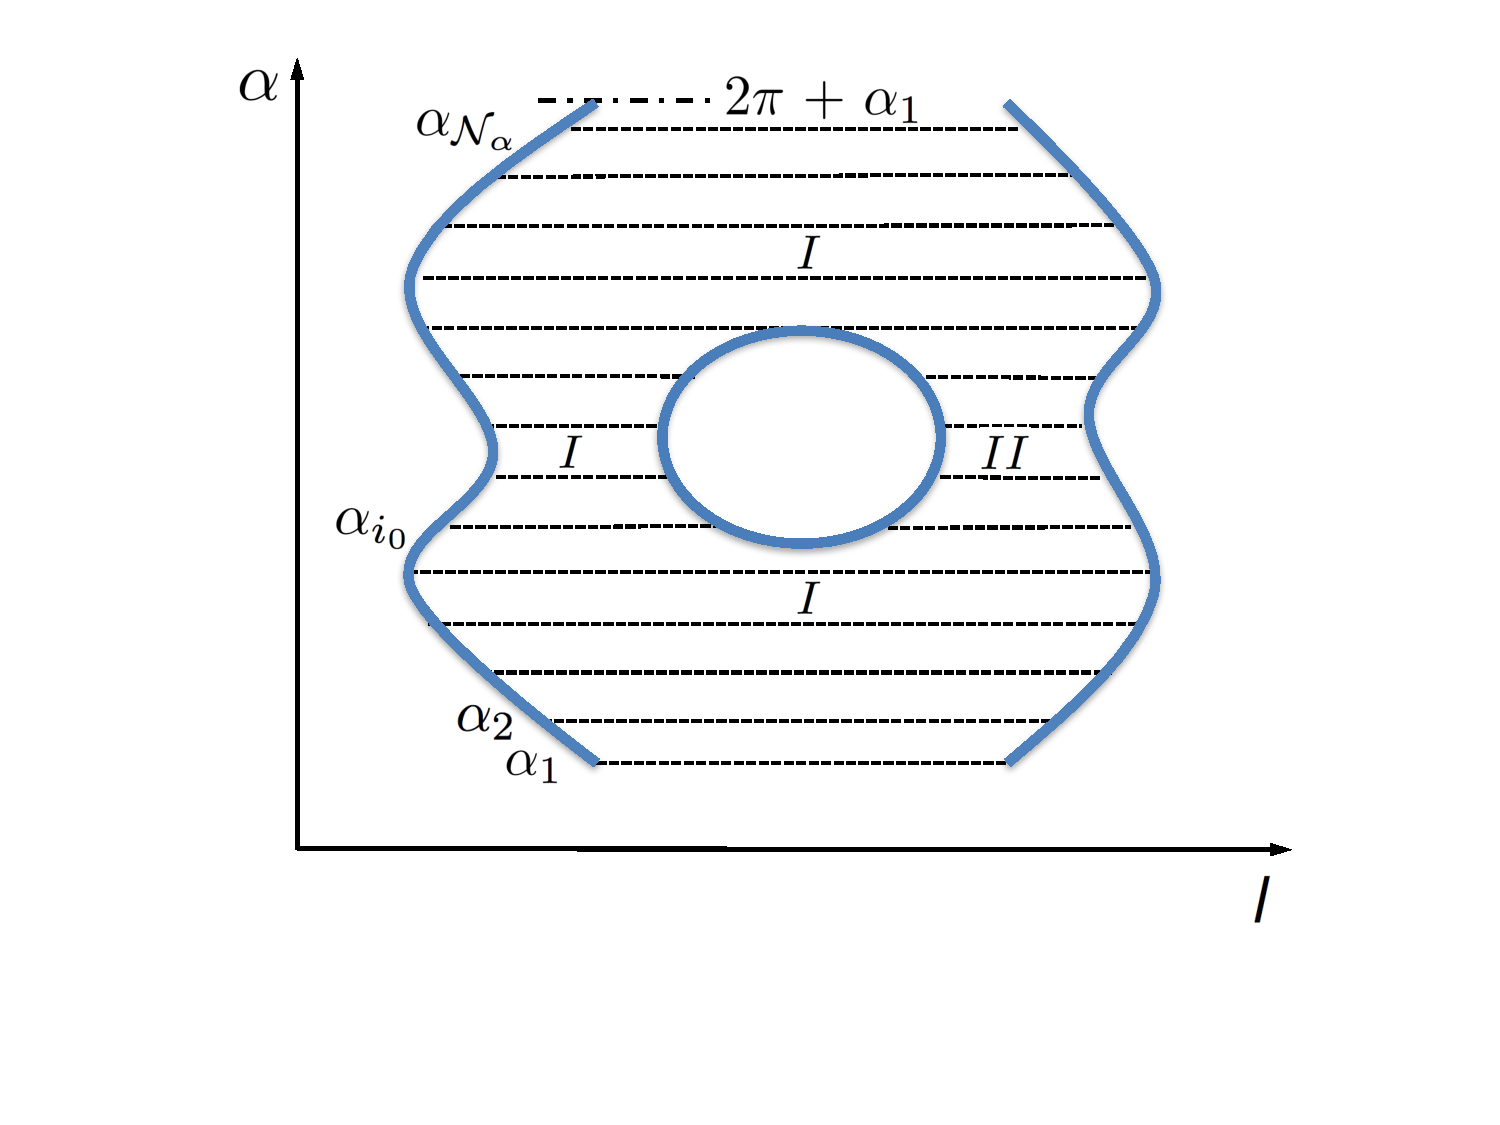
\includegraphics[angle=0,width=0.8\columnwidth]{figures/alpha_l}\vskip-1.5cm
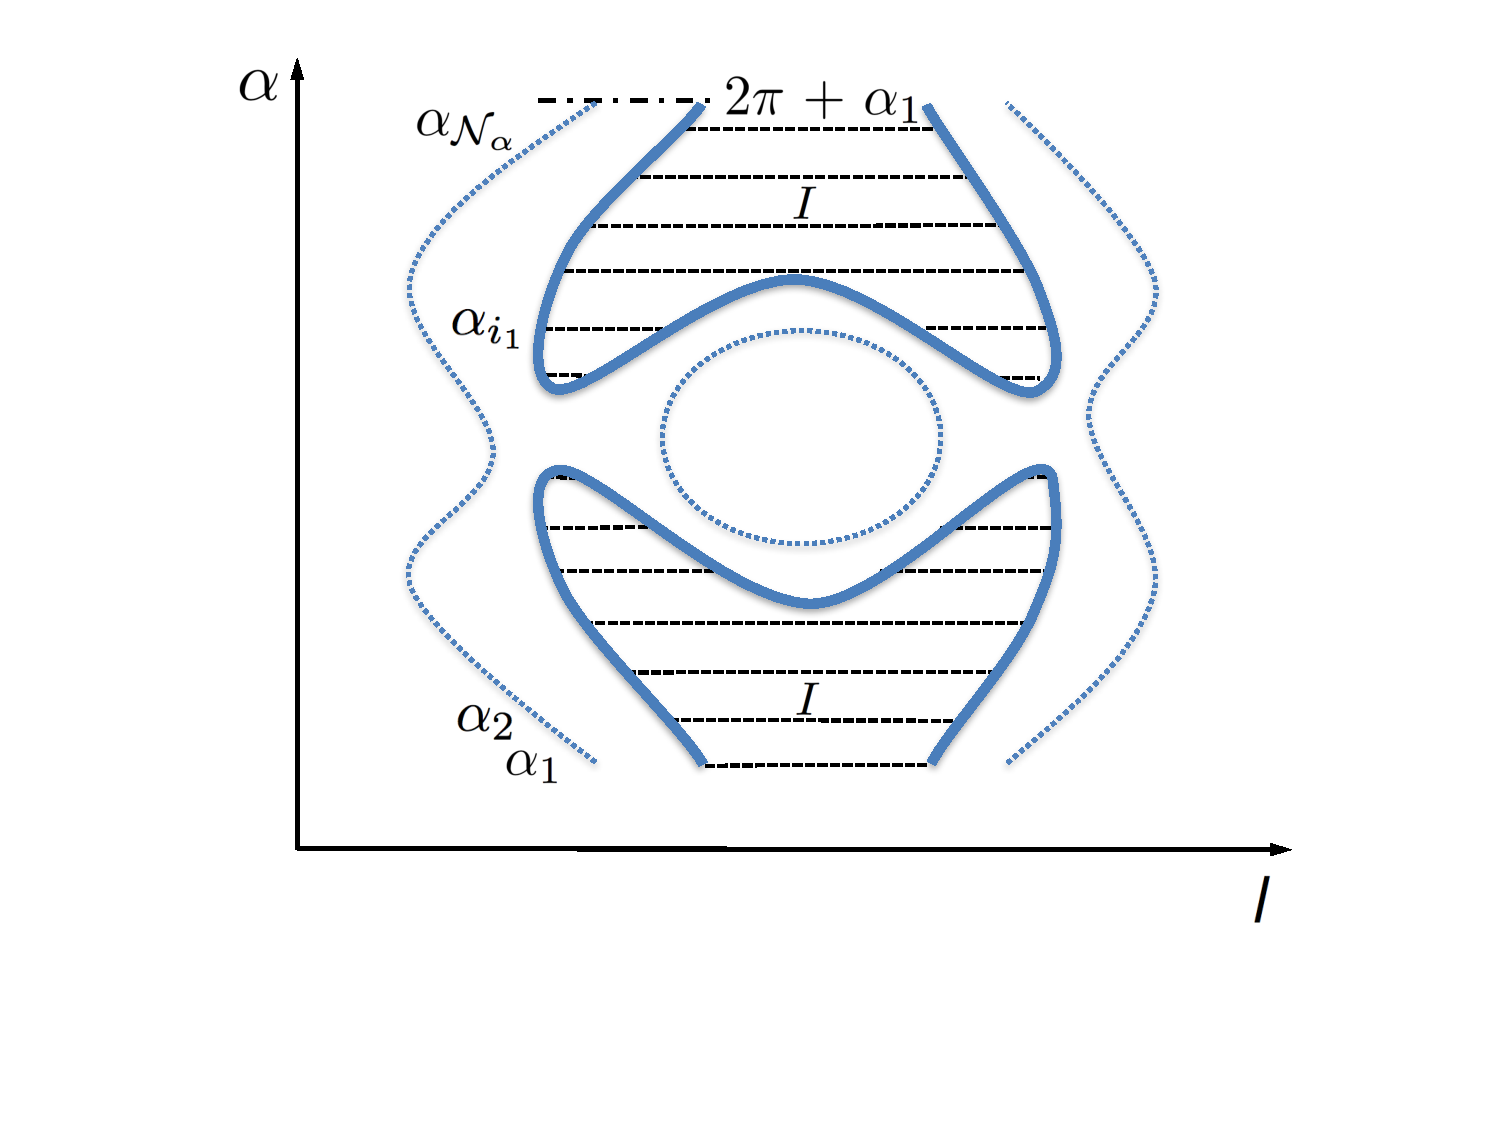
\includegraphics[angle=0,width=0.8\columnwidth]{figures/alpha_l_largelambda}\vskip-0.5cm
\caption{Top: sketch of grid in $\alpha$ space at fixed $\lambda$. The tangential derivatives are discretized as in equations~(\ref{EQ_FDALPHA}) and (\ref{EQ_BDALPHA}) except close to the limits of the grid ($\alpha_1$ and $\alpha_{{\cal{N}}_\alpha}$) and to bifurcations (e.g. $\alpha_{i_0}$); there, equations~(\ref{EQ_FDALPHAA}),~(\ref{EQ_FDALPHAB}),~(\ref{EQ_BDALPHAA}),~(\ref{EQ_BDALPHAB})  and~(\ref{EQ_BIFALPHA}) are used instead. Bottom:  sketch of grid in $\alpha$ space at larger $\lambda$ (the grid at smaller $\lambda$ is plotted for reference in dashed thin blue line). $\alpha_{i_1}$} is a point where the backward derivative is discretized as discussed in equation~(\ref{EQ_NOALPHA}).
\label{FIG_ALPHA}
\end{figure}

Let us now turn our attention to the terms with the first derivative in $\alpha$ in equation~(\ref{EQ_NDKE}), which we multiply by $v_{d,b}$:
\begin{equation}
\left(v_{d,b}I_{v_{M,\alpha}} +I_{v_E,\alpha}\right)\partial_\alpha g_b\,. 
\label{EQ_DALPHA}
\end{equation}
We represent the $\alpha$ grid at fixed $\lambda$ in figure~\ref{FIG_ALPHA} (top). In this example, there is only one well at $\alpha_1$, labelled $I$. If one moves from smaller to larger $\alpha$, a bifurcation appears in the vicinity of $\alpha_{i_0}$, with two wells labelled $I$ and $II$. At a larger value of $\alpha$, the wells merge into a single region labelled again $I$. The last point of the grid, $\alpha_{{\cal{N}}_\alpha}$, is close to $\alpha_1+2\pi$.

Non-centered finite differences with second-order accuracy are used. For a given flux-surface, for each solution of the drift-kinetic equation, the sign of the coefficient in front of $\partial_\alpha g_b$ (i.e. the direction of the flow in the $\alpha$ direction) indicates whether forward
\begin{equation}
\partial_\alpha g_b|_{i,j,w}=\frac{-g_{i+2,j,w}+4g_{i+1,j,w}-3g_{i,j,w}}{2\Delta\alpha}\,,
\label{EQ_FDALPHA}
\end{equation}
 or backward differences 
 \begin{equation}
\partial_\alpha g_b|_{i,j,w}=\frac{g_{i-2,j,w}-4g_{i-1,j,w}+3g_{i,j,w}}{2\Delta\alpha}\,,
\label{EQ_BDALPHA}
\end{equation}
should be used, with $\Delta\alpha=\alpha_{i+1}-\alpha_i$. To construct the derivatives with respect to $\alpha$ without much computational cost, we discretize separately the terms $I_{v_E,\alpha}\partial_\alpha g$ and $v_{d,b}I_{v_M,\alpha}\partial_\alpha g$ using a total of four matrices for a given flux surface. One corresponds to forward differences being used everywhere, and another one corresponds to backward differences everywhere. When solving equation ~(\ref{EQ_NDKE}), one of these two matrices will describe the $I_{v_E,\alpha}\partial_\alpha g$ term, depending on the sign of $E_r$. The other two matrices correspond to two $\lambda$ (and $w$)-dependent discretizations, in which forward (backward) differences are used according to the sign of $I_{v_{M,\alpha}}$. One of these two matrices will describe the $v_{d,b}I_{v_M,\alpha}\partial_\alpha g$ term, depending on the sign of $v_{d,b}$. Any matrix appropriate for describing equation~(\ref{EQ_DALPHA}) will thus be a linear combination of two of the four pre-calculated matrices, and a neoclassical simulation including ions and electrons and/or different values of the radial electric field will generally make use of the four of them.

Periodicity in $\alpha$ is easily imposed by replacing equation (\ref{EQ_FDALPHA}) at $i\ge{\cal{N}}_\alpha-1$ with
\begin{eqnarray}
\partial_\alpha g_b|_{{\cal{N}}_\alpha-1,j,w}&=&\frac{(g_{{\cal{N}}_\alpha,j,w}-g_{{\cal{N}}_\alpha-1,j,w})(2\pi+\alpha_1-\alpha_{{\cal{N}}_\alpha-1})}{(2\pi+\alpha_1-\alpha_{{\cal{N}}_\alpha})\Delta\alpha} \nonumber \\
&-&\frac{(g_{1,j,w}-g_{{\cal{N}}_\alpha-1,j,w})\Delta\alpha}{(2\pi+\alpha_1-\alpha_{{\cal{N}}_\alpha-1})(2\pi+\alpha_1-\alpha_{{\cal{N}}_\alpha})}\,,\label{EQ_FDALPHAA}\\
\partial_\alpha g_b|_{{\cal{N}}_\alpha,j,w}&=&\frac{(g_{1,j,w}-g_{{\cal{N}}_\alpha,j,w})(2\pi+\alpha_{2}-\alpha_{{\cal{N}}_\alpha})}{(2\pi+\alpha_{1}-\alpha_{{\cal{N}}_\alpha})\Delta\alpha} \nonumber \\
&-&\frac{(g_{2,j,w}-g_{{\cal{N}}_\alpha,j,w})(2\pi+\alpha_{1}-\alpha_{{\cal{N}}_\alpha})}{(2\pi+\alpha_{i}-\alpha_{{\cal{N}}_\alpha})\Delta\alpha}\,,\label{EQ_FDALPHAB}
\end{eqnarray}
respectively, and equation (\ref{EQ_BDALPHA}) at $i\le 2$ with
\begin{eqnarray}
\partial_\alpha g_b|_{2,j,w}&=&-\frac{(g_{1,j,w}-g_{2,j,w})(\alpha_{{\cal{N}}_\alpha}-\alpha_2-2\pi)}{(\alpha_{{\cal{N}}_\alpha}-\alpha_1-2\pi)\Delta\alpha} \nonumber \\
&+&\frac{(g_{{\cal{N}}_\alpha,j,w}-g_{2,j,w})\Delta\alpha}{(\alpha_{{\cal{N}}_\alpha}-\alpha_2-2\pi)(\alpha_{{\cal{N}}_\alpha}-\alpha_1-2\pi)}\,,\label{EQ_BDALPHAA}\\
\partial_\alpha g_b|_{1,j,w}&=&-\frac{(g_{{\cal{N}}_\alpha,j,w}-g_{1,j,w})(\alpha_{{\cal{N}}_\alpha-1}-\alpha_1-2\pi)}{(\alpha_{{\cal{N}}_\alpha}-\alpha_1-2\pi)\Delta\alpha} \nonumber \\
&+&\frac{(g_{{\cal{N}}_\alpha-1,j,w}-g_{1,j,w})(\alpha_{{\cal{N}}_\alpha}-\alpha_1-2\pi)}{(\alpha_{{\cal{N}}_\alpha-1}-\alpha_1-2\pi)\Delta\alpha}\,,
\label{EQ_BDALPHAB}
\end{eqnarray}
respectively. We note  that, since $\iota$ is generally irrational, $2\pi+\alpha_1-\alpha_{{\cal{N}}_\alpha}$ will e.g. be slightly smaller than $\Delta\alpha$


We also note that bifurcations do not pose a problem for $\alpha$-derivatives, due to $g_b$ being continuous in $\alpha$. For example, in the vicinity of $\alpha_{i_0}$ in figure~\ref{FIG_ALPHA} (top) the forward derivative is discretized
\begin{eqnarray}
\partial_\alpha g_b|_{i_0-2,j,I}&=&\frac{-g_{i_0-2,j,I}+4g_{i_0-1,j,I}-3g_{i_0,j,I}}{2\Delta\alpha}\nonumber\\
&=&\frac{-g_{i_0-2,j,I}+4g_{i_0-1,j,I}-3g_{i_0,j,II}}{2\Delta\alpha}\,,\nonumber\\
\partial_\alpha g_b|_{i_0-1,j,I}&=&\frac{-g_{i_0-1,j,I}+4g_{i_0,j,I}-3g_{i_0+1,j,I}}{2\Delta\alpha}\nonumber\\
&=&\frac{-g_{i_0-1,j,I}+4g_{i_0,j,II}-3g_{i_0+1,j,II}}{2\Delta\alpha}\,,\nonumber\\
\partial_\alpha g_b|_{i_0,j,I}&=&\frac{-g_{i_0,j,I}+4g_{i_0+1,j,I}-3g_{i_0+2,j,I}}{2\Delta\alpha}\,,\nonumber\\
\partial_\alpha g_b|_{i_0,j,II}&=&\frac{-g_{i_0,j,II}+4g_{i_0+1,j,II}-3g_{i_0+2,j,II}}{2\Delta\alpha}\,,\nonumber\\
\partial_\alpha g_b|_{i_0+1,j,I}&=&\frac{-g_{i_0+1,j,I}+4g_{i_0+2,j,I}-3g_{i_0+3,j,I}}{2\Delta\alpha}\,,\nonumber\\
\partial_\alpha g_b|_{i_0+1,j,II}&=&\frac{-g_{i_0+1,j,II}+4g_{i_0+2,j,II}-3g_{i_0+3,j,II}}{2\Delta\alpha}\,,\nonumber\\
\partial_\alpha g_b|_{i_0+2,j,I}&=&\frac{-g_{i_0+2,j,I}+4g_{i_0+3,j,I}-3g_{i_0+4,j,I}}{2\Delta\alpha}\,,\nonumber\\
\partial_\alpha g_b|_{i_0+2,j,II}&=&\frac{-g_{i_0+2,j,II}+4g_{i_0+3,j,II}-3g_{i_0+4,j,I}}{2\Delta\alpha}\,,\nonumber\\
\partial_\alpha g_b|_{i_0+3,j,I}&=&\frac{-g_{i_0+3,j,I}+4g_{i_0+4,j,I}-3g_{i_0+5,j,I}}{2\Delta\alpha}\,,\nonumber\\
\partial_\alpha g_b|_{i_0+3,j,II}&=&\frac{-g_{i_0+3,j,II}+4g_{i_0+4,j,I}-3g_{i_0+5,j,I}}{2\Delta\alpha}\,,
\label{EQ_BIFALPHA}
\end{eqnarray}
where continuity of $g_b$ has been used in the first two expressions of equation~(\ref{EQ_BIFALPHA}). Equivalent expressions can be obtained for the backward derivative.

One final caveat has to be made. In an omnigenous magnetic field, the contours of minimum $B$ on a flux surface must encircle the plasma (toroidally, poloidally, or helically). This is not true for a generic stellarator, in which local minima of $B$ exist on the flux surface. Close to these minima, moving in $\alpha$ at constant large $\lambda$ is not always possible, as these trajectories may not exist. This situation is illustrated in figure~\ref{FIG_ALPHA} (bottom), at $\alpha_{i_1}$. At, $\alpha_{i_1}$, instead of equation (\ref{EQ_BDALPHA}), we use
 \begin{equation}
\partial_\alpha g_b|_{i_1,j,w}=\frac{g_{i_1-2,j_0,w}-4g_{i_1-1,j,w}+3g_{i_1,j,w}}{2\Delta\alpha}\,.\label{EQ_NOALPHA}
\end{equation}
and we have implemented two models: in one, $\lambda_{j_0}$ is the value of $\lambda$ closest to $\lambda_j$ in which trajectories exist for all $\alpha$; in the second model, $\lambda_{j_0}$ is the closest value of $\lambda$ in which trajectories exist at $\alpha_{i_0-2}$. The relative differences between the two models are smaller than e.g. the error bars of~\DKES~in figure~\ref{FIG_D11PROF}. We note that (with different manifestations for other choices of velocity coordinates) an incorrect treatment of this kind of particles is common to all existing radially local codes.
%
%\
%
%~~~~~~~~~~~~~~~$\left(I_{v_{M,\alpha}}+\frac{1}{v_{d,b}}I_{v_{E,\alpha}}\right)\partial_\alpha +\frac{\nu_{\lambda,b}}{v_{d,b}} \partial_\lambda \nu\partial_\lambda $~~~~~~~~~$g_b$~~~~~~~$\left[I_{v_{M,\psi}} \right.+\left.\frac{1}{v_{d,b}}I_{v_{E,\psi}}\right] F_{M,b}\Upsilon_b$
%
%
%\[
%\begin{bmatrix}
%    \dots       & \dots & \dots & \dots &\dots \\
%    \dots       & \dots & \dots & \dots & \dots \\
%    \dots       & \dots & \dots & \dots & \dots \\
%    \dots       & \dots & \dots & \dots & \dots     
%\end{bmatrix}
%\cdot
%\begin{bmatrix}
%    \dots  \\
%    \dots  \\
%    \dots  \\
%    \dots 
%\end{bmatrix}
%=
%\begin{bmatrix}
%    \dots  \\
%    \dots  \\
%    \dots  \\
%    \dots 
%\end{bmatrix}
%\]
%
%\


For each of the species $b$, we end up with an equation that is linear in $g_b$ and can be written as a linear problem in matrix form. The matrix that represents
\begin{equation}
\left(I_{v_{M,\alpha}}+\frac{1}{v_{d,b}}I_{v_{E,\alpha}}\right)\partial_\alpha +\frac{\nu_{\lambda,b}}{v_{d,b}} \partial_\lambda \nu\partial_\lambda 
\end{equation}
is square with approximately ${\cal{N}}_\lambda\times {\cal{N}}_\alpha$ elements per row, and sparse, with $\sim 6$ non-zero elements per row: between 3 and 5 for the $\alpha$ derivatives, and typically 2 additional points for the collision operator. Although their relative weight varies with $\nu_{\lambda,b}$, $v_{d,b}$ and $\partial_\psi\varphi_0$, the non-zero elements are always at the same position for a given flux-surface, which can be used to save computing time, by using the four pre-computed matrices described above.

We solve the linear problem with a direct solver from the {\ttfamily PETSc} library~\citep{petsc-efficient,petsc-web-page,petsc-user-ref} based on LU factorization. The reason is that the matrix is not large enough to require iterative methods, and reusing the LU factorization greatly accelerates the solution of the quasineutrality equation, as discussed in \S\ref{SEC_SOLQN}.

%%%%%%%%%%%%%%%%%%%%%%%%%%%%%%%%%%%%%%%%%%%%%%%%%%%%%%%%%%%%%%%%%%%%%%%%%%%%%%%%%%%%%%%%%%%%%%%%%%%%%%%%%%%%%%%%%%%

\section{Solution of the quasineutrality equation}\label{SEC_SOLQN}

%%%%%%%%%%%%%%%%%%%%%%%%%%%%%%%%%%%%%%%%%%%%%%%%%%%%%%%%%%%%%%%%%%%%%%%%%%%%%%%%%%%%%%%%%%%%%%%%%%%%%%%%%%%%%%%%%%%

We will solve the quasineutrality equation by means of a response matrix approach (similar methods are used in gyrokinetics for the calculation of the electrostatic potential fluctuations~\citep{kotschenreuther1995response}). Let us first rewrite equations (\ref{EQ_NDKE}) and~(\ref{EQ_QNFINAL}) making explicit the dependence on $\varphi_1$:

\begin{eqnarray}
\left(I_{v_{M,\alpha}} +\frac{I_{v_{E,\alpha}}}{v_{d,b}}\right)\partial_\alpha g_b-\frac{\nu_{\lambda,b}}{v_{d,b}} \partial_\lambda I_\nu \partial_\lambda g_b ~~~~~~~~~~~~~~~~~~~~~~~~~~~~~~~~~~~& &\nonumber\\=\left(I_{v_{M,\psi}}-\int_{l_{b_1}}^{l_{b_2}} \frac{\mathrm{d}l}{\sqrt{1-\lambda B}}\frac{B_\theta\partial_\zeta \varphi_1 - B_\zeta\partial_\theta \varphi_1}{|B_\zeta+\iota B_\theta|} \right) F_{M,b}\Upsilon_b\,,\label{EQ_DKEPHI1}\\
\left(\frac{Z_i}{T_i}+\frac{1}{T_e}\right)\varphi_1 =\frac{2\pi}{en_e}\sum_b Z_b \int_0^\infty\mathrm{d} v \int_{B^{-1}_{{\rm max}}}^{B^{-1}}\mathrm{d}\lambda\frac{v^3 B}{|v_\parallel |}g_b\,.~~~~~~~~~~~~~~~\label{EQ_QNPHI1}
\end{eqnarray}
It can be observed that equation~(\ref{EQ_DKEPHI1}) is linear in $\varphi_1$, and therefore the response of the distribution function $g_b$ (and of its velocity integral) of species $b$ to certain $\varphi_1$ can be calculated as a superposition of the responses to a complete set of harmonics that parametrize $\varphi_1(\theta,\zeta)$. We can perform this parametrization efficiently thanks to the Fast Fourier Transform, using ${\cal{N}}=2(2{\cal{N}}_n+1)({\cal{N}}_m+1)$ coefficients:
\begin{equation}
\varphi_1(\theta,\zeta) =\sum_{-{\cal{N}}_n<n<{\cal{N}}_n} \sum_{0<m<{\cal{N}}_m} \left(\varphi^{(c)}_{mn}\cos(m\theta+Nn\zeta)+\varphi^{(s)}_{mn}\sin(m\theta+Nn\zeta)\right)\,
\label{EQ_FFTPHI1}
\end{equation}
(the grid defined in \S\ref{SEC_GRID} is not uniform in $\theta$, so an interpolation is done before the Fourier transform). We can now denote $u_k(\theta,\zeta)$ each of the ${\cal{N}}$ basis elements (e.g. $\cos(\theta+2N\zeta)$) and the combined system of drift-kinetic and quasineutrality equation can be symbolically written as
\begin{eqnarray}
\pmb{\varphi_1} = \pmb{\varphi_1^{0}} + \mathbf{A}\pmb{\varphi_1}\,,
\end{eqnarray}
where $\pmb{\varphi_1}$ is a vector whose ${\cal{N}}$ components are the coefficients of the expansion of $\varphi_1$ in equation~(\ref{EQ_FFTPHI1}) and $\mathbf{A}$ is a generally dense ${\cal{N}}\times{\cal{N}}$ matrix. In this linear, system, the right-hand side $\pmb{\varphi_1^{0}}$ can be obtained by solving equation~(\ref{EQ_DKEPHI1}) for all the kinetic species with $\varphi_1=0$, inserting the solution into equation~(\ref{EQ_QNPHI1}) and then Fourier-transforming the result following equation~(\ref{EQ_FFTPHI1}). Next, we fill the matrix $\mathbf{A}$: the \textit{kth} row is obtained by solving equation~(\ref{EQ_DKEPHI1}) with $\varphi_1= u_k$,  inserting the solution into equation~(\ref{EQ_QNPHI1}), Fourier-transforming and then substracting $\pmb{\varphi_1^{0}}$ from the result. Once $\pmb{\varphi_1^{0}}$ and $\mathbf{A}$ have been filled, the new linear system can easily be solved, e.g. using a new LU decomposition, to obtain $\pmb{\varphi_1}$, i.e., the set of coefficients $\varphi^{(c)}_{mn}$ and $\varphi^{(s)}_{mn}$ that parametrize the solution to quasineutrality. Finally, since the response of $g_b$ to every basis element has already been computed, a simple linear combination yields the distribution function that is solution of the drift-kinetic and quasineutrality equations, without requiring an additional solve of the former.

In summary, the drift-kinetic equation is solved a total of ${\cal{N}}+1$ times (for each species), but LU factorization is done once (for each value of $v$). The linearity of the system of equations due to the smallness of $\varphi_1$, together with the method that we have chosen for solving the drift-kinetic equation, yields a large reduction of the computing time needed to solve the system of equations: the code is roughly ${\cal{N}}$ faster (with ${\cal{N}}$  ranging from 100 to 1000), with respect to an equivalent code that allowed the particle orbits be modified by $\varphi_1$.


%\section{Workflow}
%
%The main loop is contained in file {\ttfamily low\_collisionality.f90} (subroutine {\ttfamily CALC\_LOW\_COLLISIONALITY}), and it takes the following steps:
%
%\begin{itemize}
%\item Find and characterize all the wells (see \S\ref{SEC_WCOEF}).
%\item Create a grid in $\alpha$, then in $(\zeta,\theta)$).
%\item Set a grid in $\lambda$.
%\item Create a global grid, with one point per value of $\lambda$, $\alpha$, and well label for a given $\alpha$.
%\item For each point ($\zeta,\theta,\lambda$), determine the well number and the position in the absolute grid.
%\item Find the neighbours in $\lambda$.
%\item Calculate the coefficients of the drift-kinetic equation (i.e. bounce-integrals) for each point of the absolute grid.
%\item Find the neighbours in $\alpha$.
%\item Prepare the matrix for the linear system.
%\item For each case (corresponding to different velocity):
%\begin{itemize}
%\item Fill the matrix and right-hand-side vector.
%\item Solve the linear problem and obtain the monoenergetic distribution function.
%\item Calculate the monoenergetic contribution to the flux and $\varphi_1$ by  integrating it the velocity space and taking the flux-surface-average.
%\end{itemize}
%\end{itemize}
%



